\documentclass[12pt]{article}
\usepackage{amsmath,amsthm,amssymb,dsfont,polynom}
\usepackage[pdftex]{graphicx}

\graphicspath{{images/}}

\usepackage[margin = 1.0in]{geometry}
\usepackage{fancyhdr}
\usepackage{hyperref}
\pagestyle{fancy}
\lhead{Francis Pich\'e}

\thispagestyle{empty}


\newtheorem{problem}{Problem} 
\theoremstyle{definition} 
\newtheorem*{solution}{Solution}

\usepackage{listings}
\usepackage{color}

\definecolor{dkgreen}{rgb}{0,0.6,0}
\definecolor{gray}{rgb}{0.5,0.5,0.5}
\definecolor{mauve}{rgb}{0.58,0,0.82}

\lstset{frame=tb,
  language= Python,
  aboveskip=3mm,
  belowskip=3mm,
  showstringspaces=false,
  columns=flexible,
  basicstyle={\small\ttfamily},
  numbers=none,
  numberstyle=\tiny\color{gray},
  keywordstyle=\color{blue},
  commentstyle=\color{dkgreen},
  stringstyle=\color{mauve},
  breaklines=true,
  breakatwhitespace=true,
  tabsize=3
}


\begin{document}
\title{COMP361 FlashPoint Project Sketch}
\author{T. Azim-zada, N. Amiraslan, F. Pich\'e, SC. Haw, A. Bedard, A. Gupta}
\date{\today}
\maketitle
\newpage
\tableofcontents
\newpage

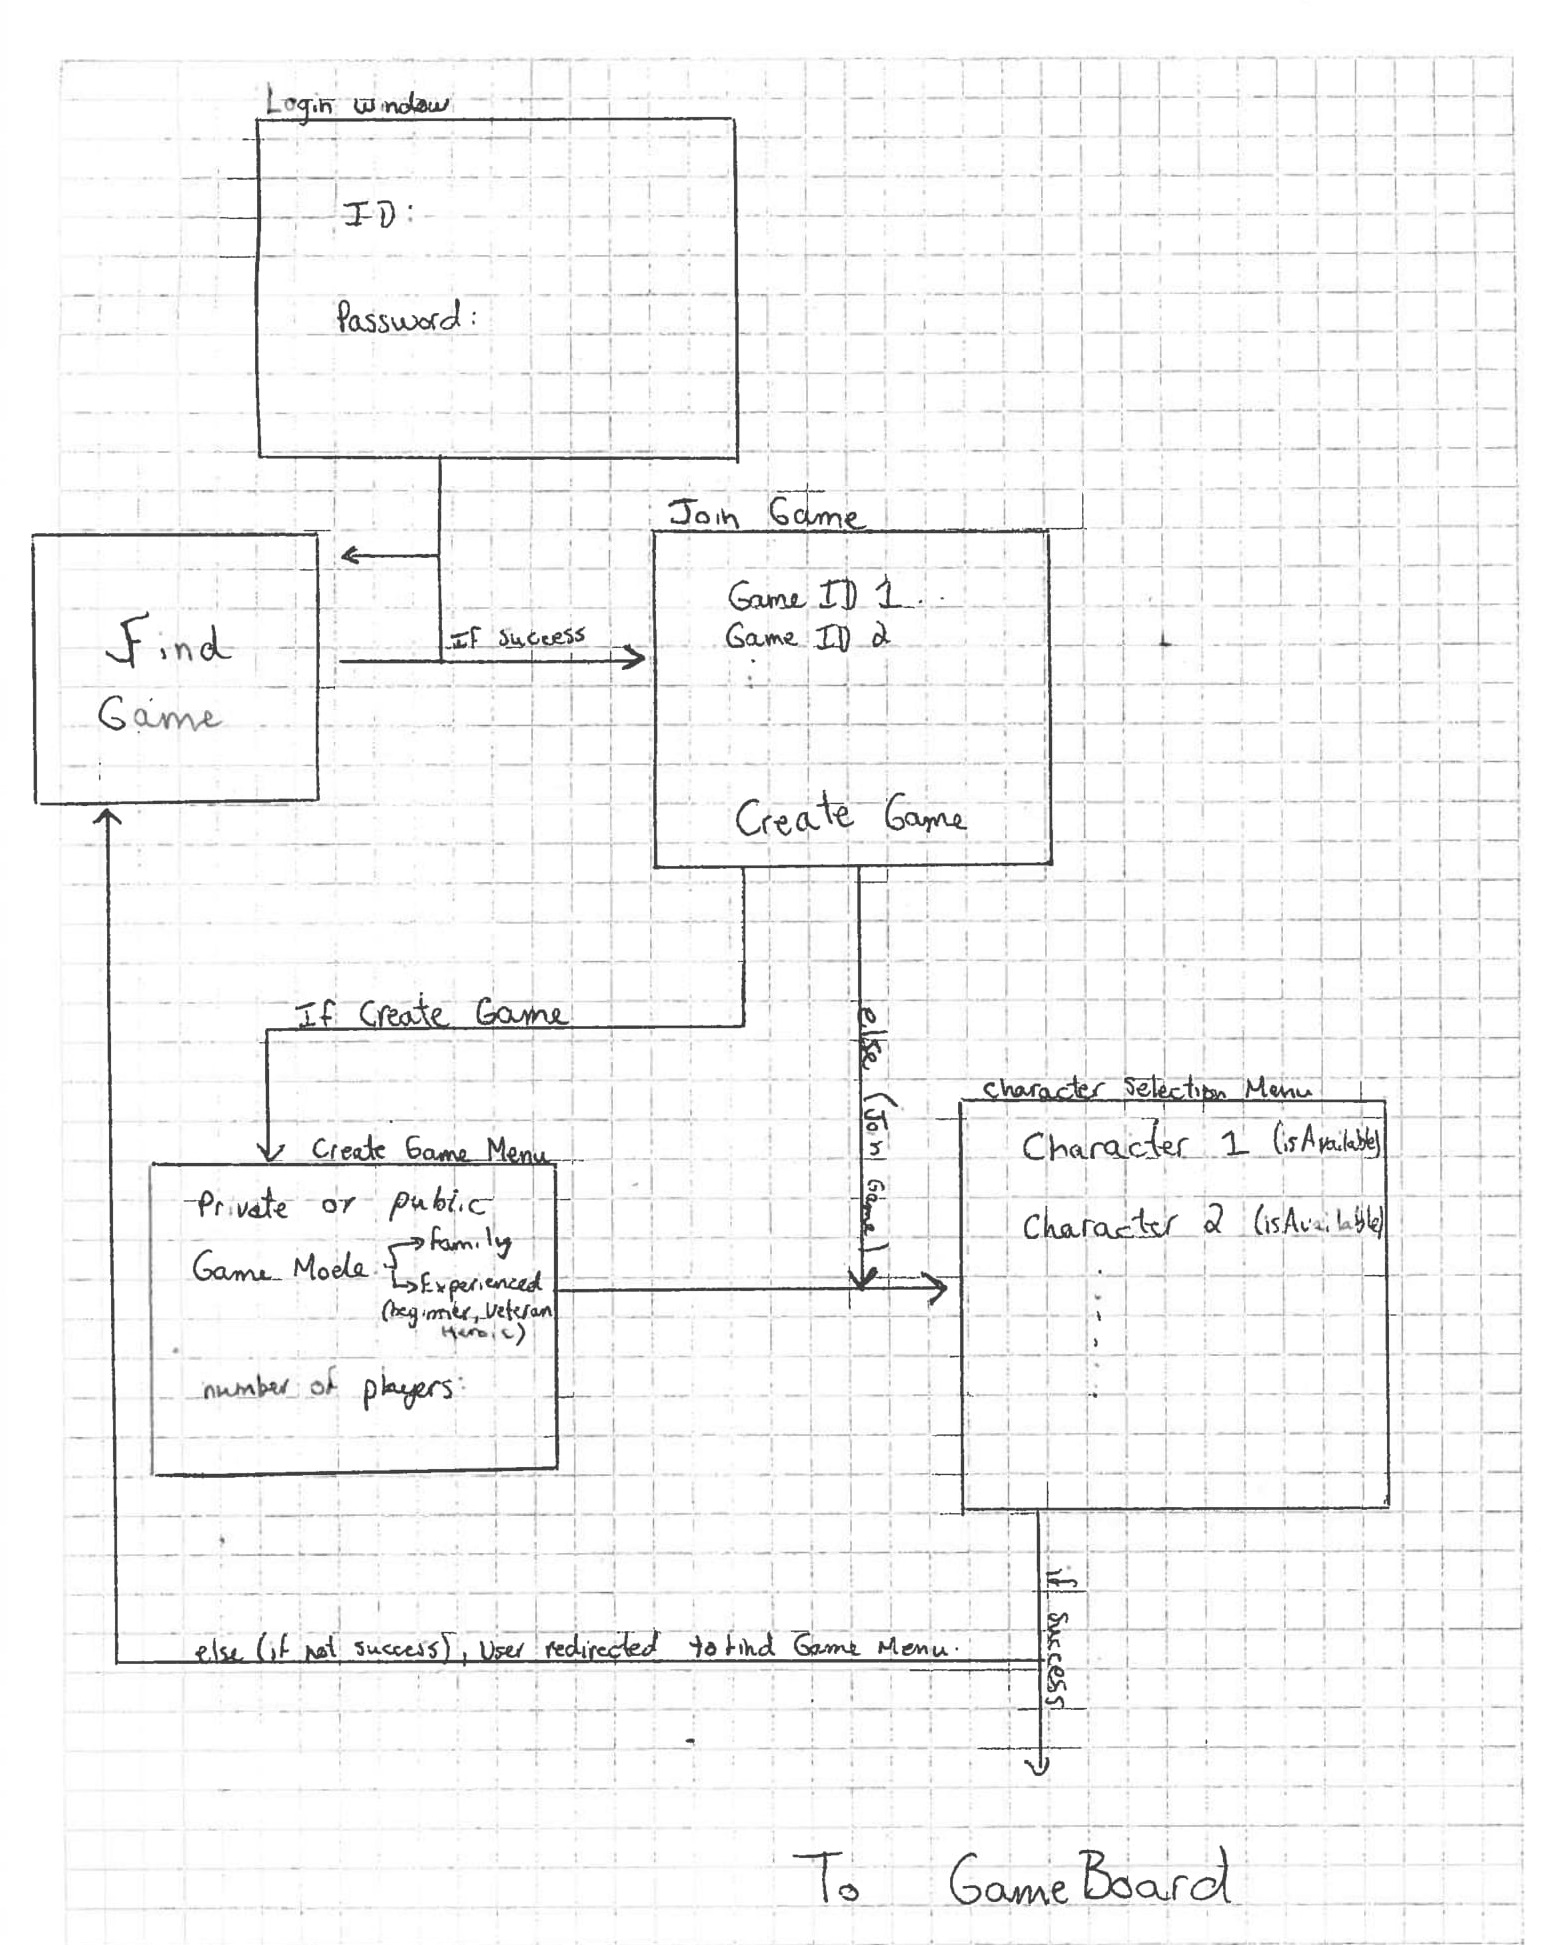
\includegraphics[scale=0.5]{LoginFindGame}
\part{Login}
User is prompted for credentials to authenticate to server. Once the login is successful, the \textbf{Find Game} screen is opened.

\part{Find Game}
\textbf{Find Game}: When pressed, the user will be presented with existing games which can be joined. If the user selects an existing game, they will be placed in the character selection screen. They also have the option to create a new game. The new game creation window will prompt the user for:
\begin{itemize}
	\item Whether the game is private (password protected) or public.
	\item The game mode (Family or Experienced)
	\item If Experienced, choose difficulty level (Recruit, Veteran, Heroic)
	\item The number of players required to start the game.
\end{itemize} 
Once the game has been created, the user is taken to the character selection screen.
\\ \linebreak
The user is then prompted to choose a character from the available characters (Not already selected by another user). The user is then taken to the main game board.
\\ \linebreak
The game starts when the number of users required to start the game are in the main game board.

\part{Main Game}
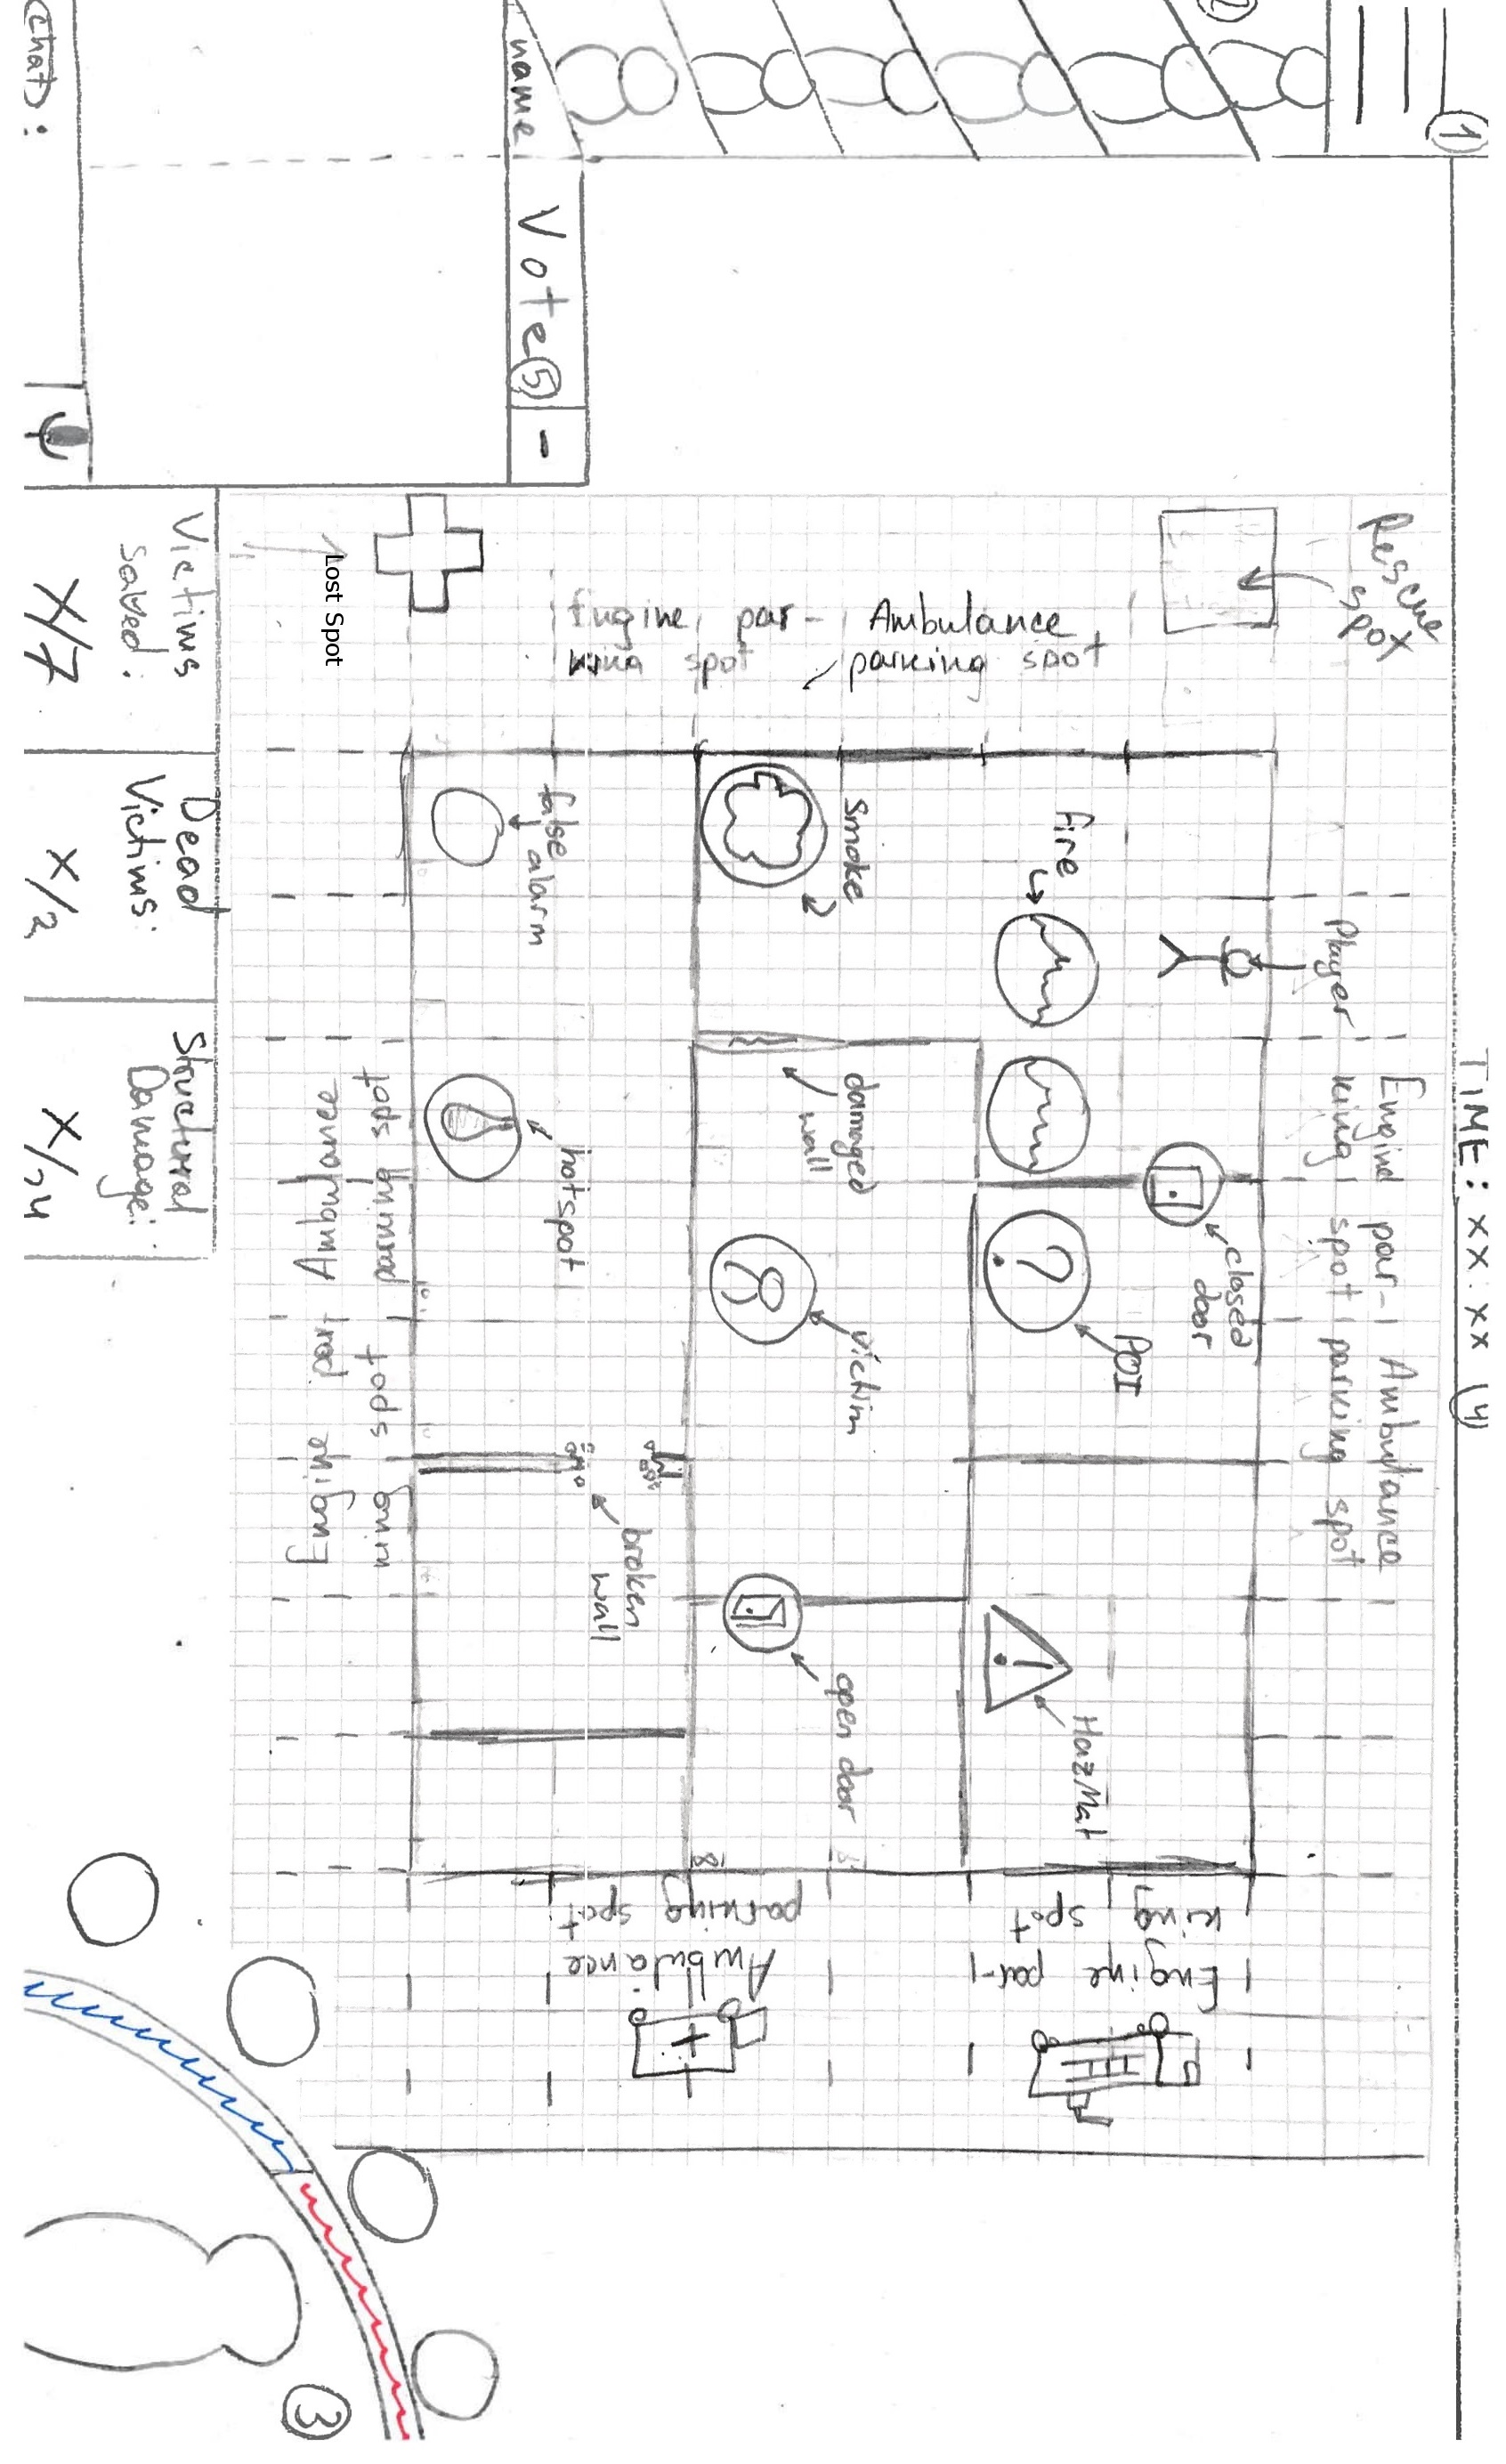
\includegraphics[width=\textwidth, height=\textheight]{HUD}
\section*{Menu}
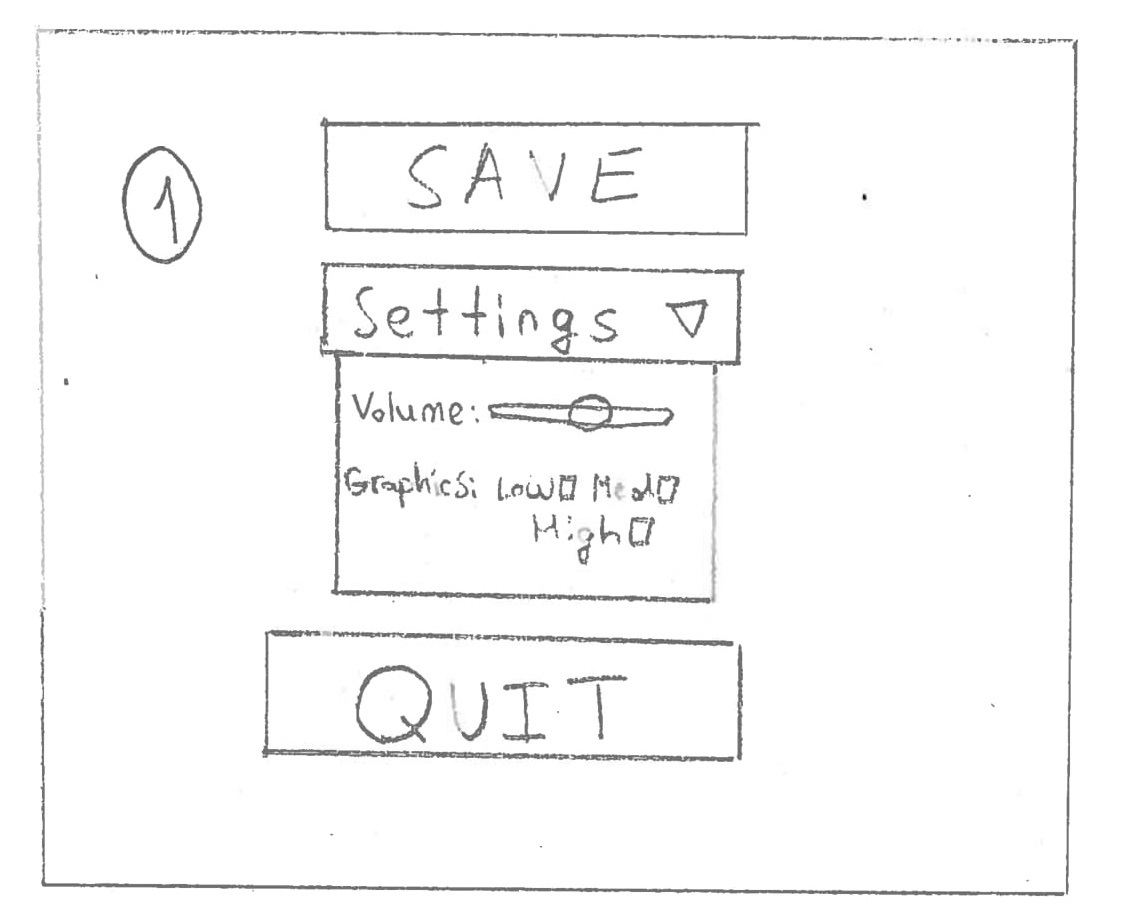
\includegraphics[scale=0.5]{MainMenu}\\
$^1$ When clicked, the menu window will open. The menu window contains the following options:
\begin{itemize}
	\item Save: Save the game state to the server for future loads. If this button is never pressed, the game will be lost when all players have quit.
	\item Settings: Open a menu for changing generic sound and video settings.
	\item Quit: Exit the game.
\end{itemize}

\section*{Game State}
$^2$ When hovered over, this will display information about another user. This includes AP points, the users login name and name of special character.
\\ \linebreak
Along the bottom, the following statistics are displayed:
\begin{itemize}
	\item Victims saved $x/7$
	\item Victims lost $x/3$
	\item Total structural damage $x/24$
\end{itemize}

$^3$ Displays information about the users character. Current AP (in blue) and special AP (in red) is in the bars. The outer circles are reserved for character special abilities.
\\ \linebreak
$^4$ The time left for the current players turn.
\\ \linebreak

\section*{Communication}
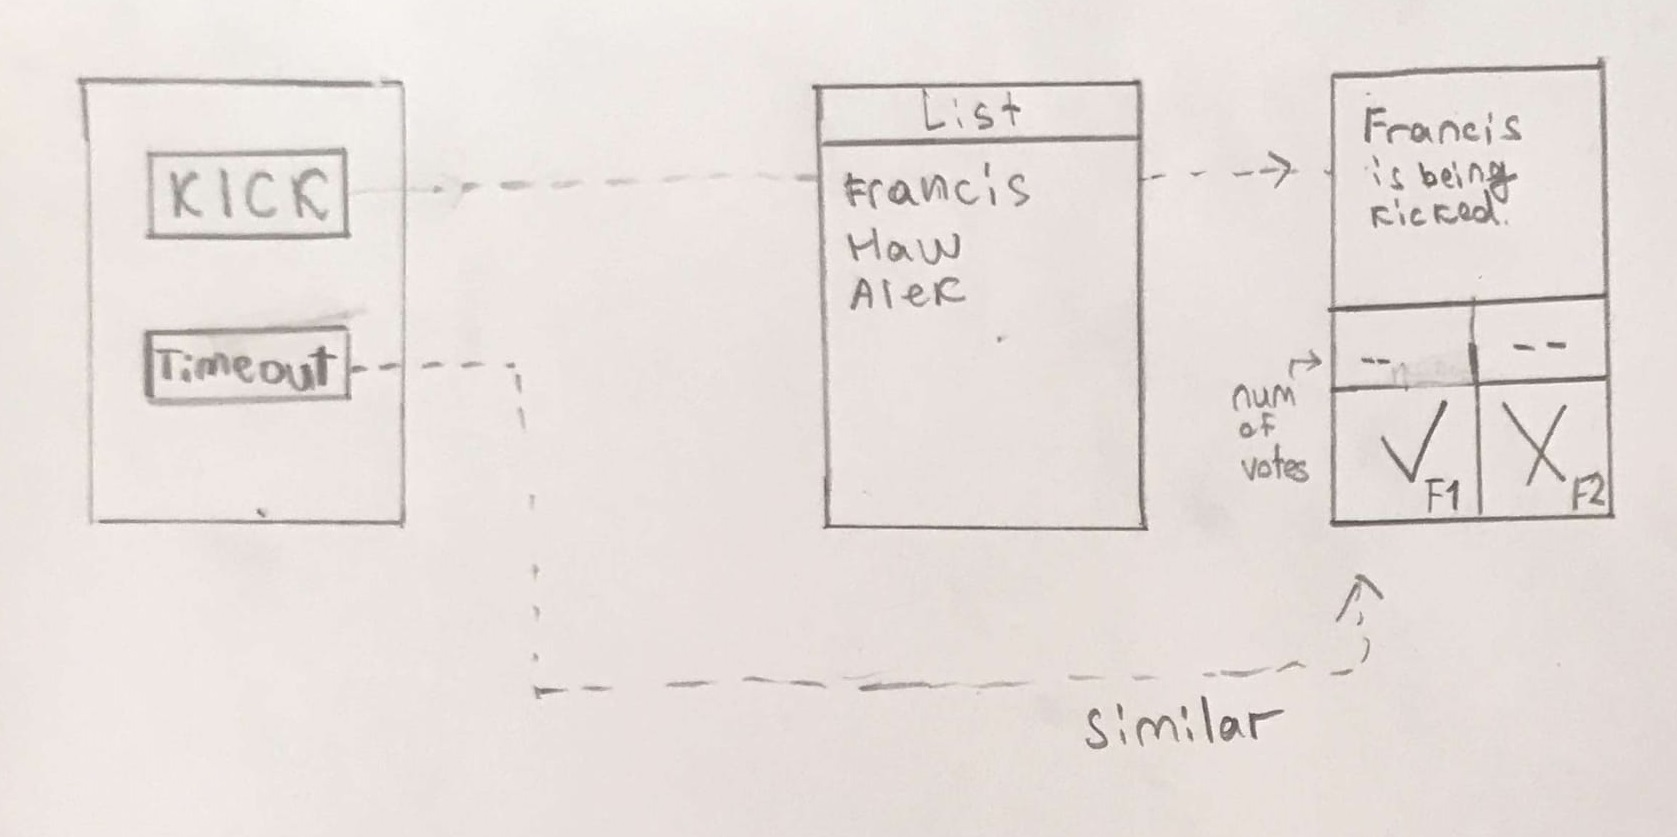
\includegraphics[scale=0.3]{Vote}\\
$^5$ When clicked, the Vote menu is opened. Here the user will be prompted with:
\begin{itemize}
	\item Kick user: Call vote to remove a player from the game.
	\item Time-out: Call vote to pause the game for a pre-determined length of time.
\end{itemize}
The chat box can send messages to all other users in text form. There is also a mute-microphone button for voice chat.
\\ \linebreak
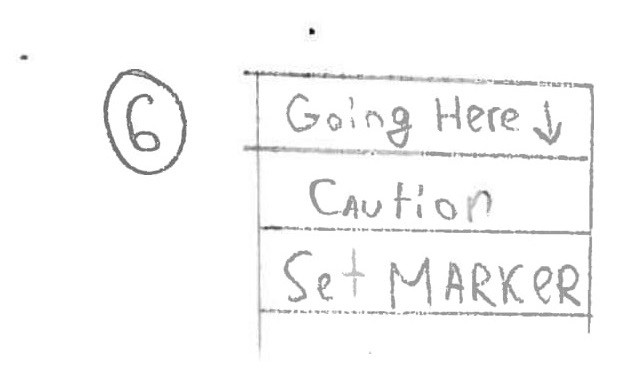
\includegraphics[scale=0.5]{PingMenu}\\
$^6$ When a special button is pressed and held, combined with a click on a location on the map, a small box will appear to prompt the user for a type of Ping. The selection will be communicated to all other users and a marker will appear on the map in the location of the click. The markers can be one of: 
\begin{itemize}
	\item Going here: Communicate that the user intends to move to the specified location.
	\item Caution: Communicate to other users that a location requires attention.
	\item Set marker: Set a generic marker on the map. 
\end{itemize}
These can be placed by a player regardless of whether it is their turn or not.
\section*{Execute Turn}
To indicate that is is a given users turn, all non-playing users character icon will be faded grey. Only the user who's currently executing a turn will be in color. 
\\ \linebreak
A highlighted region around the users character to indicate which tiles are within range. The user can then click on a portion of the highlighted region to open the options for that tile. Depending on what the tile contains, there would be different options.
\\ \linebreak
This process can be repeated until the user does not have enough AP to complete another task within range.
\\ \linebreak
The players character icon will also overlay a "End Turn" text, which can be clicked to end the turn.
\\ \linebreak

\end{document}